\documentclass{article}
\usepackage[utf8]{inputenc}
\usepackage[russian]{babel}
\usepackage{geometry}
\usepackage{indentfirst}
\usepackage{amsmath}
\usepackage{float}
\usepackage[14pt]{extsizes}
\usepackage{graphicx}

\geometry{a4paper,left=30mm,top=30mm,bottom=30mm,right=30mm}
\setcounter{secnumdepth}{0} 

\begin{document}

\begin{titlepage}
    \begin{center}
	{\small \sc Московский государственный университет \\имени М.~В.~Ломоносова\\
	Факультет вычислительной математики и кибернетики\\
	Кафедра оптимального управления\\}
	\vfill
	\vspace{5cm}
	{\Large \bf Отчёт по практикуму}\\
	~\\
	{\large \bf Программа для решения краевых задач методом продолжения по параметру{}}\\
	~\\
	~\\
	~\\
	~\\
	~\\
	\vspace{5cm}
	\begin{flushright}
	    \textbf{Преподаватели:}$\quad$ Аввакумов С.Н.\\ Киселев Ю.Н.\\ Дряженков А.А.\\
	    \vspace{0,5cm}
        \textbf{Выполнил:}$\quad$	Иванов Максим, группа 313
	\end{flushright}
    \end{center}
    \begin{center}
	\vfill
	{\small Москва\\2021}
    \end{center}
\end{titlepage}

% Автоматически генерируем оглавление на отдельной странице
\tableofcontents

\newpage

\section{Постановка и описание задачи}

\subsection{Цель работы}

Реализовать программу для решения кравевых задач методом продолжения по параметру в среде \textit{Matlab}.
Программа должна решать краевую задачу выбранным методом и показывать результаты своей работы на графиках.

\section{Реализация задачи}

\subsection{Информация о среде}

Программа реализована в среде \textit{Matlab 2014b}. Использовались всевозможные средства среды для реализации пользовательского интерфейса, аналитического решения возникающих задач, чтения и записи файлов.

\subsection{Описание интерфейса}

Программа имеет несколько окон. Основное окно содержит семь блоков элементов интерфейса.

Первый блок - меню в верхней части окна. Меню имеет четыре пункта: <<Управление>>, <<Примеры>>, <<Помощь>> и <<О программе>>. 

В первом пункте собраны команды для сохранения введённой задачи (<<Сохранить задачу>>, комбинация горячих клавиш \textit{Ctrl+S}), которая открывает стандартное системное окно сохранения файлов и загрузки ранее введённой задачи (<<Загрузить задачу>>, комбинация горячих клавиш \textit{Ctrl+O}), которая открывает стандартное системное окно открытия файлов. (Рис. \ref{ris:menu})

\begin{figure}[!h]
\center{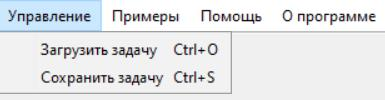
\includegraphics[scale=1]{menu.jpg}}
\caption{Меню программы}
\label{ris:menu}
\end{figure}

Второй пункт меню открывает окно с библиотекой примеров, в котором представлен список примеров из учебного пособия [4] и присутствуют две кнопки для открытия примера и закрытия окна. (Рис. \ref{ris:examples})

\begin{figure}[!h]
\center{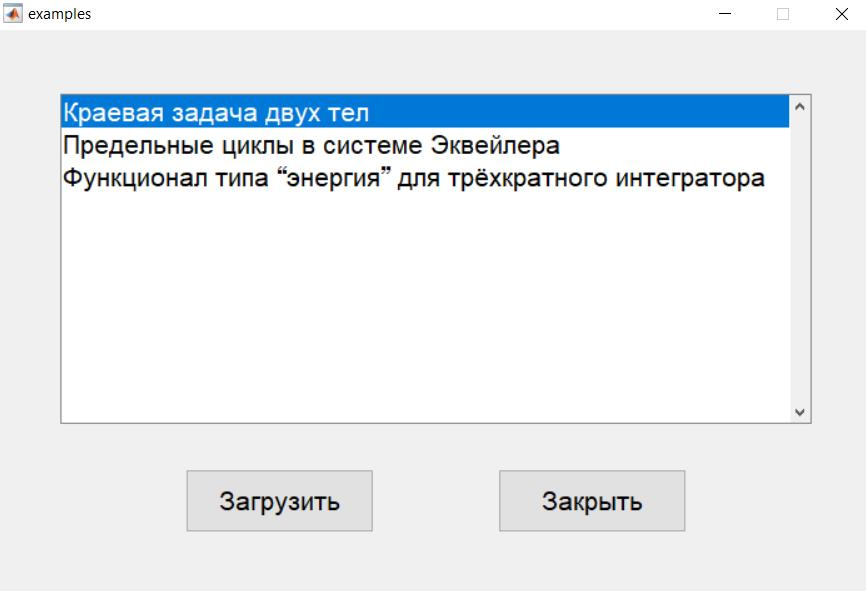
\includegraphics[scale=0.75]{examples.jpg}}
\caption{Окно <<Примеры>>}
\label{ris:examples}
\end{figure}

Третий пункт меню открывает окно <<Помощь>> (Рис. \ref{ris:help}). 

\begin{figure}[!h]
\center{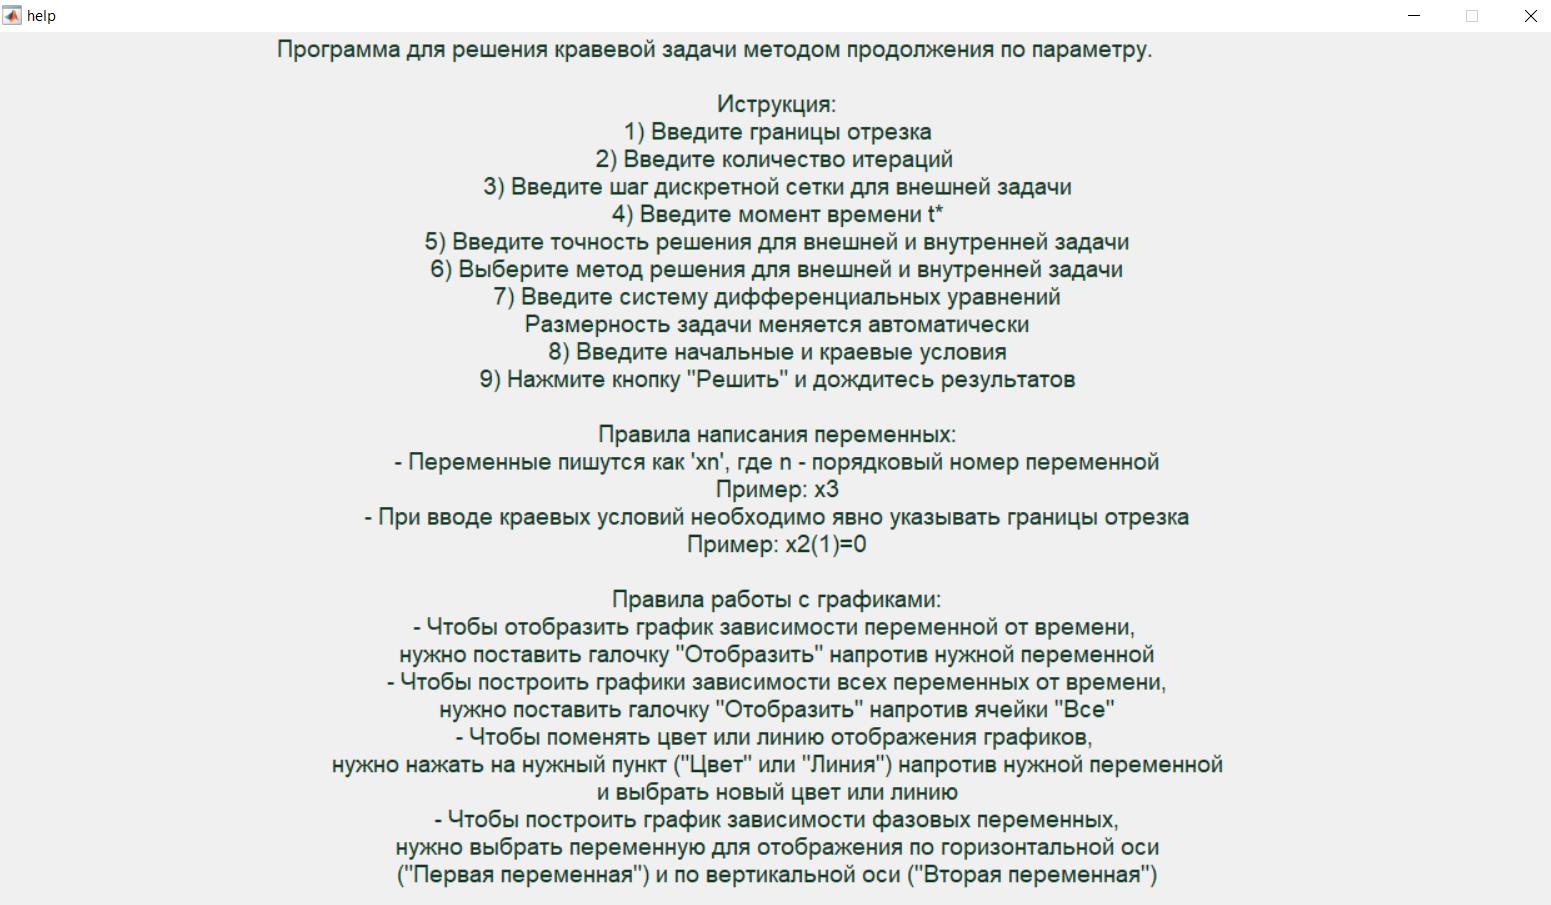
\includegraphics[scale=0.5]{help.jpg}}
\caption{Окно <<Помощь>>}
\label{ris:help}
\end{figure}

Четвёртый пункт меню открывает окно <<О программе>> (Рис. \ref{ris:about}).

\begin{figure}[!h]
\center{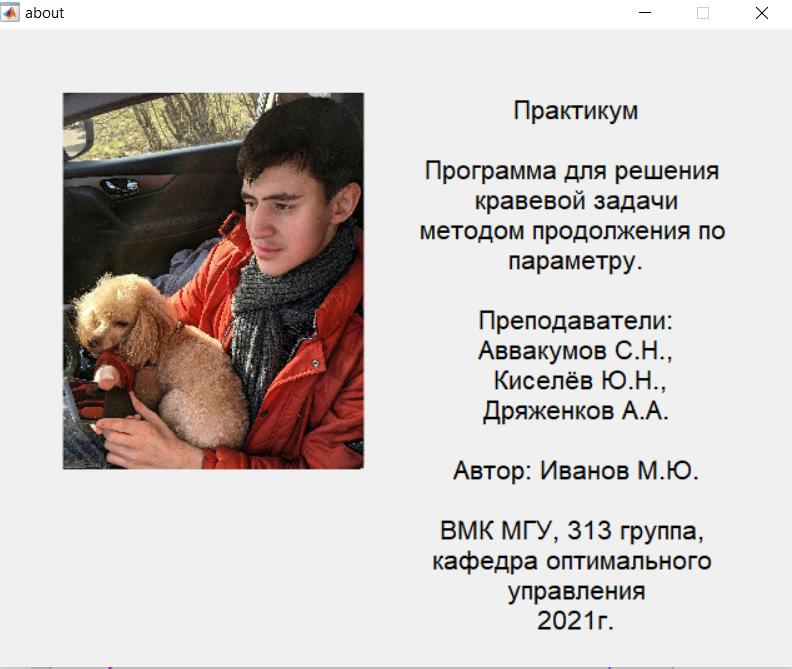
\includegraphics[scale=0.75]{about.jpg}}
\caption{Окно <<О программе>>}
\label{ris:about}
\end{figure}


Далее основное окно делится еще на шесть блоков.
Блоки <<Ввод краевой задачи>> и <<Ввод краевых условий>> предназначены для ввода системы дифференциальных уравнений и краевых условий. Данные блоки содержат таблицы, в которые необходимо вводить саму краевую задачу. Размерность таблиц регулируется автоматически, новые поля появляются при необходимости. (Рис. \ref{ris:main})

Блок <<Настройки>> и <<Вектор начальных условий p0>> предназначен для ввода настроек метода. Пользователь может ввести начало отрезка, конец отрезка, количество итераций, шаг сетки внешней задачи, момент времени t*, точность и метод решения для внешней и внутренней задачи и вектор начальных условий p0. (Рис. \ref{ris:main})

Блок <<Решение>> содержит кнопки для вычисления решения, очистки данных и просмотра результатов. Также под кнопками показывается время выполнения вычислений.

Последний блок позволяет написать название и комментарий к введенной задаче. (Рис. \ref{ris:main})

\begin{figure}[!h]
\center{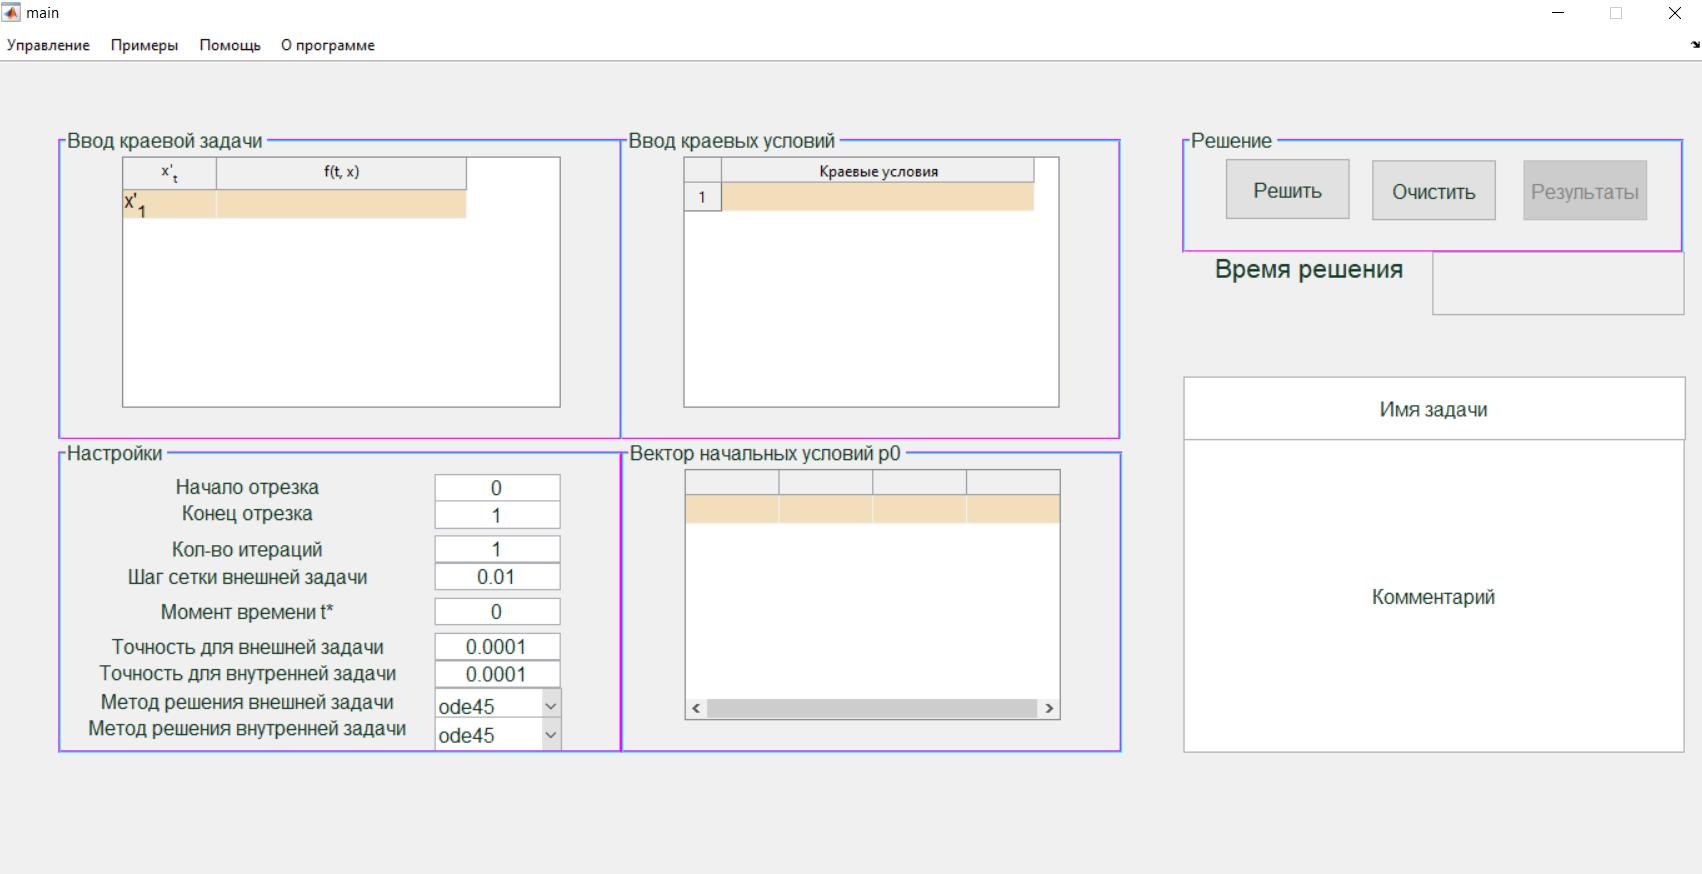
\includegraphics[scale=0.37]{main.jpg}}
\caption{Основное окно}
\label{ris:main}
\end{figure}

\newpage

Окно <<Результаты>> содержит три блока элементов интерфейса. 

Первый блок содержит таблицу, в которой показаны значения всех переменных в каждой точке временной сетки. (Рис. \ref{ris:sol})

Второй блок содержит координатную ось для вывода графиков зависимости переменных от времени и таблицу, расположенную под нею, в которой можно выбрать переменные для построения графика, выбирать для каждого из них цвет и тип линий. (Рис. \ref{ris:sol})

Третий блок содержит координатную ось для вывода графиков зависимости фазовых переменных. Первая перменная отвечает за ось абцисс, а вторая - за ось ординат. (Рис. \ref{ris:sol})

\begin{figure}[!h]
\center{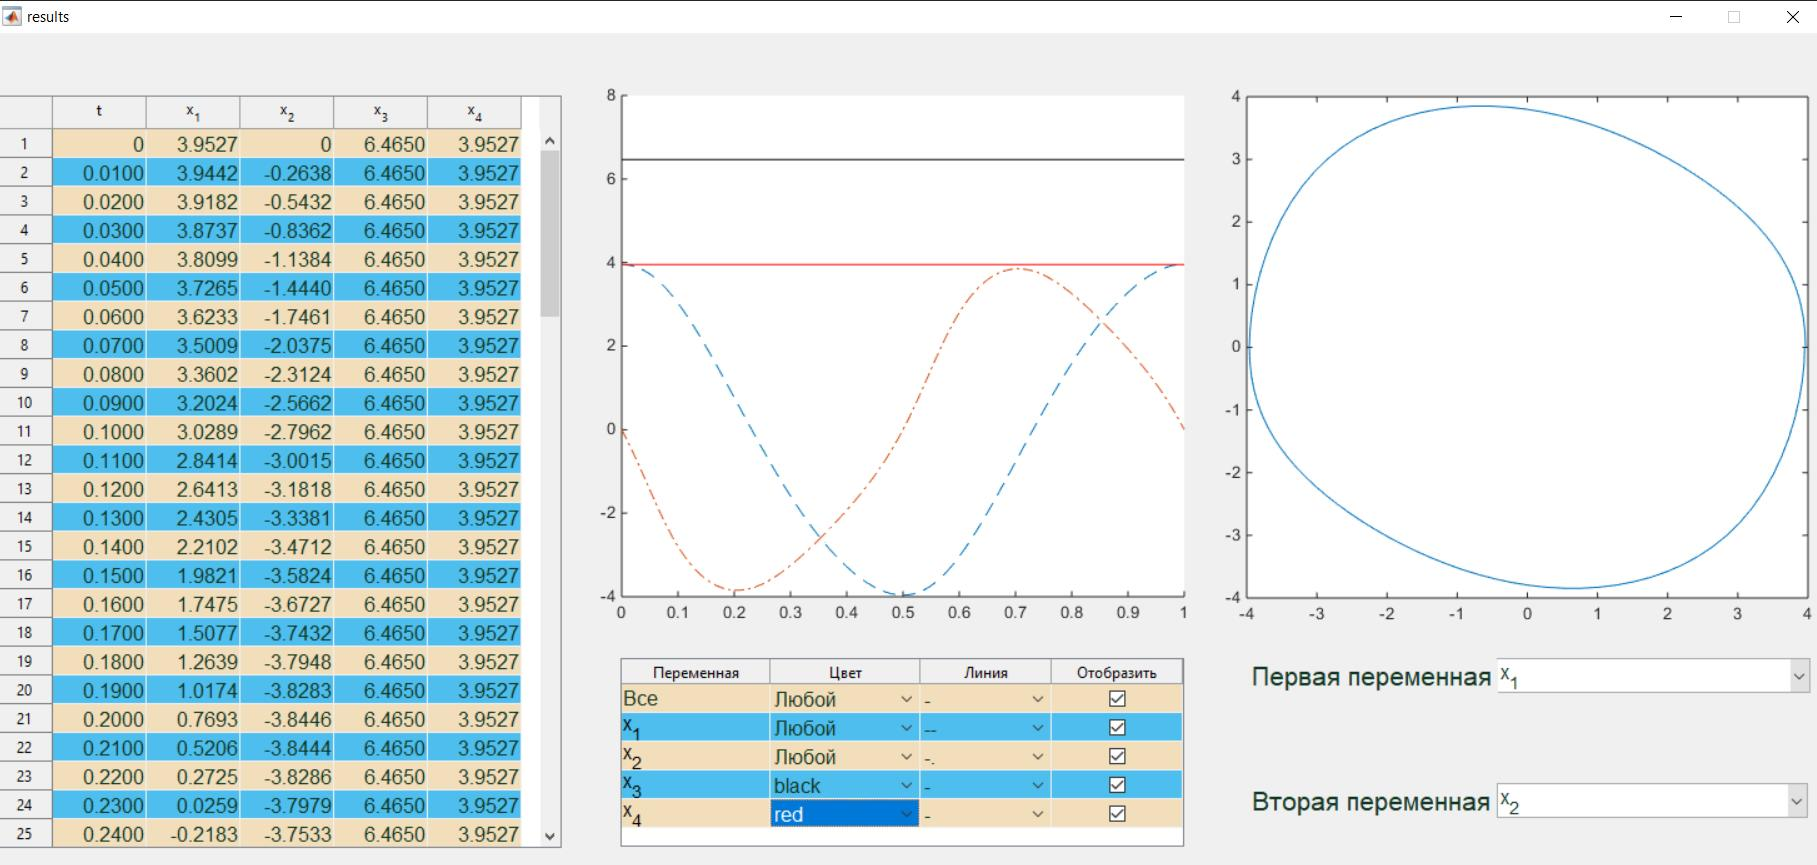
\includegraphics[scale=0.37]{sol.jpg}}
\caption{Окно решения для задачи <<Предельные циклы в системе Эквейлера>>}
\label{ris:sol}
\end{figure}

\newpage

\section{Метод продолжения по параметру}

Рассмотрим краевую задачу 
$$
	\dot{x}=f(t,x), \; R(x(a),x(b))=0, \;t \in [a,b], \; x \in E^n. \eqno(1)
$$ 

\noindent Здесь $f(t,x): E^1 \times E^n \mapsto E^n, \; R(x,y): E^n \times E^n  \mapsto E^n$ являются гладкими векторными функциями. Предполагая существование решения краевой задачи (1), обсудим алгоритмические вопросы поиска её решения. Решение краевой задачи можно свести к некоторому нелинейному векторному уравнению в $E^n$. Выберем некоторую точку $t_* \in [a, b]$ и рассмотрим задачу Коши
$$
	x=f(t,x), \; x|_{t=t_*} = p \in E^n. \eqno(2)
$$

\noindent Свобода выбора точки $t_*$ может быть полезна для вычислительной
практики. Пусть

$$
	x(t,p), \; a \le t \le b. \eqno(3)
$$

\noindent --- решение задачи Коши (2). Предполагается продолжимость решения (3) на весь отрезок $[a, b]$ для любого $p$. Начальное значение параметра $p \in E^n$ ищется из условий выполнения векторного граничного условия в задаче (1), т.е. искомое $p$ является решением уравнения
$$
	\Phi(p) \equiv R(x(a, p), x(b, p)) = 0. \eqno(4)
$$

\noindent Итак, краевая задача (1) сведена к конечному векторному уравнению (4). Далее к уравнению (4) применяется метод продолжения. Матрица $\Phi'(p)$ определяется равенством
$$
	\Phi'(p)=R'_x\frac{\partial x(a,p)}{\partial p} + R'_y\frac{\partial x(b,p)}{\partial p}
$$

\noindent Здесь $(n \times n)$ --- матрицы $R'_x (x, y), \; R'_y (x, y)$ вычисляются вдоль решения (3), т.е. при $x = x(a, p), \; y = x(b, p)$. Введём обозначение
$$
	X(t, p) \equiv \frac{\partial x(t, p)}{\partial p}
$$
\noindent для $(n \times n)$---матрицы производных решения (3) по начальному условию. Матрица $X(t,p)$ определяется дифференциальным уравнением в вариациях
$$
	\dot{X}=AX, \; X|_{t=t_*} = I, \; a \le t \le b,
$$

\noindent где $A = A(t, p) \equiv f'_x (t, x)|_{x=x(t,p)}$ есть $(n \times n)$---матрица, $I$---единичная матрица. Основная задача Коши схемы продолжения по параметру имеет вид
$$
	\text{\textbf{IVP:}} \;\;\; \frac{dp}{d\mu} = -[\Phi'(p)]^{-1}\Phi(p_0), \; p(0) = p_0, \; 0 \le \mu \le 1, \eqno(5)
$$
где
\begin{align*}
	&\Phi(p) = R(x(a,p),x(b,p)),\\
	&\Phi' (p) = R'_x (x(a, p), x(b, p))X (a, p) + R'_y (x(a, p), x(b, p))X (b, p).
\end{align*}

\indent Для одновременного вычисления векторной функции $x(t, p)$ и матричной функции $X(t,p)$ может быть записана следующая векторно-матричная задача Коши

$$
\begin{cases}
	\dot{x}=f(t, x), &x|_{t=t_*}=p,\\
	\dot{X}=f'_x(t, x)X, &X|_{t=t_*}=I, \; a \le t \le b.
\end{cases} \eqno (6)
$$

\noindent Задачу Коши (5) будем называть внешней задачей, задачу Коши (6) --- внутренней задачей. Таким образом, предлагается итерационный процесс для решения рассматриваемой краевой задачи (1) на основе внешней задачи (5) и внутренней задачи (6). На одном шаге итерационного процесса выполняется решение внешней задачи (5), в ходе решения которой происходит многократное обращение к решению внутренней задачи Коши (6) при различных значениях параметра $p$.

\newpage

\section{Результаты работы}

В данном разделе показаны результаты работы программы для примеров из раздела <<Примеры>>.

Все замеры произведены с точностями для внешней и внутренней задач 0.0001.

\subsection{Краевая задача двух тел}

$$
\begin{cases}
	\dot{x}_1=x_3, &x_1(0)=a_1, \;x_1(T)=b_1,
	\\
	\dot{x}_2=x_4, &x_2(0)=a_2, \;x_2(T)=b_2,
	\\
	\dot{x}_3=-x_1(x_1^2+x_2^2)^{-3/2}, 
	\\
	\dot{x}_4=-x_2(x_1^2+x_2^2)^{-3/2}.
\end{cases}	
$$

\noindent Для данных $
T = 7, \; a_1 = 2, \;a_2 = 0, \;b_1 = 1.0738644361, \;b_2 = -1.0995343576,
$
при выборе параметра $t_* = 0$, для начального приближения 
$
p_0 = [2, 0, 0.5, -0.5].
$

Методы решения внешней и внутренней задачи: метод Рунге-Кутта 4-5 порядка.

Время решения: 140 секунд при 3 итерациях.

\begin{figure}[!h]
\center{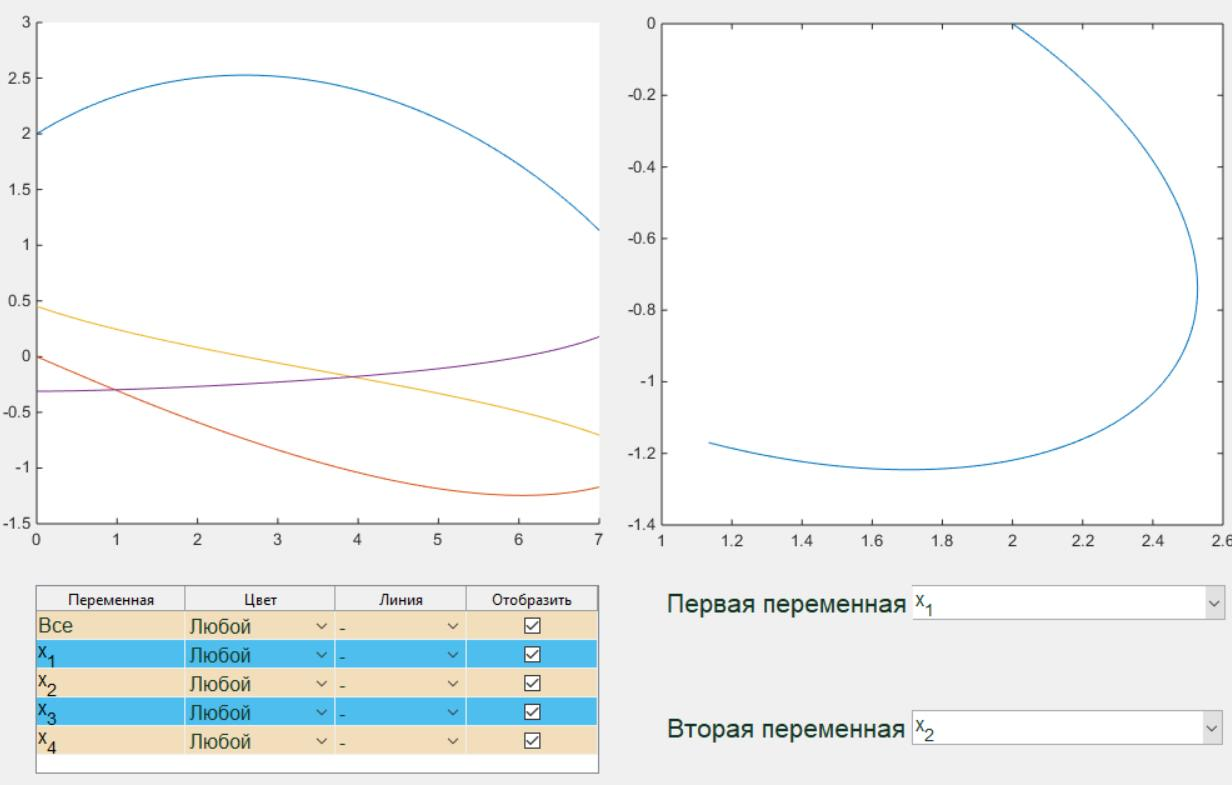
\includegraphics[scale=0.55]{task_1.jpg}}
\caption{Результаты решения задачи <<Краевая задача двух тел>>}
\label{ris:task1}
\end{figure}

\subsection{Предельные циклы в системе Эквейлера}

$$
\begin{cases}
\dot{x}_1=x_3x_2, &x_1(0)=x_4(0), \;x_1(1)=x_4(1),
\\
\dot{x}_2=x_3(-x_1+sin(x_2)), &x_2(0)=0, \;x_2(1)=0,
\\
\dot{x}_3=0, 
\\
\dot{x}_4=0.
\end{cases}	
$$

\noindent При выборе параметра $t_* = 0$, для начального приближения 
$
p_0 = [2, 0, 2\pi, 2].
$

Методы решения внешней и внутренней задачи: метод Рунге-Кутта 4-5 порядка.

Время решения: 225 секунд при 5 итерациях.

\begin{figure}[H]
\center{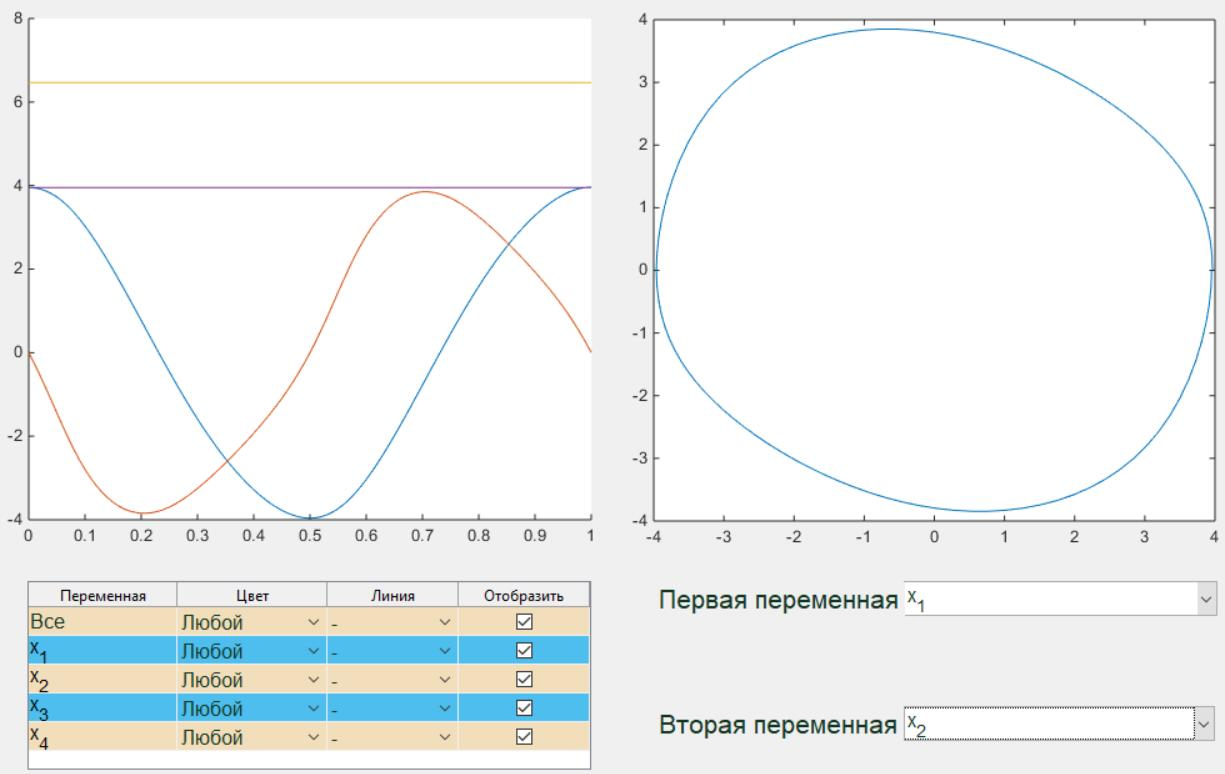
\includegraphics[scale=0.55]{task_2.jpg}}
\caption{Результаты решения задачи <<Предельные циклы в системе Эквейлера>>}
\label{ris:task2}
\end{figure}

\newpage

\subsection{Функционал типа "энергия" для трёхкратного интегратора}

$$
\begin{cases}
\dot{x}_1=x_2,
\\
\dot{x}_2=x_3,
\\
\dot{x}_3=\frac{1}{2}(\sqrt{\nu + (x_6+1)^2}-\sqrt{\nu + (x_6-1)^2}), 
\\
\dot{x}_4=0,
\\
\dot{x}_5=-x_4,
\\
\dot{x}_6=-x_5.
\end{cases}	
$$

\noindent При выборе параметров $t_* = 3.275, \; \nu = 10^{-10}$, для начального приближения 
$$
p_0 = [0, 0, 0, -2.9850435834, 4.8880088678, -2.9083874537].
$$

Метод решения внешней задачи: метод Эйлера.

Метод решения внутренней задачи: метод Рунге-Кутта 4-5 порядка.

Время решения: 33 секунды при 5 итерациях.

\begin{figure}[!h]
\center{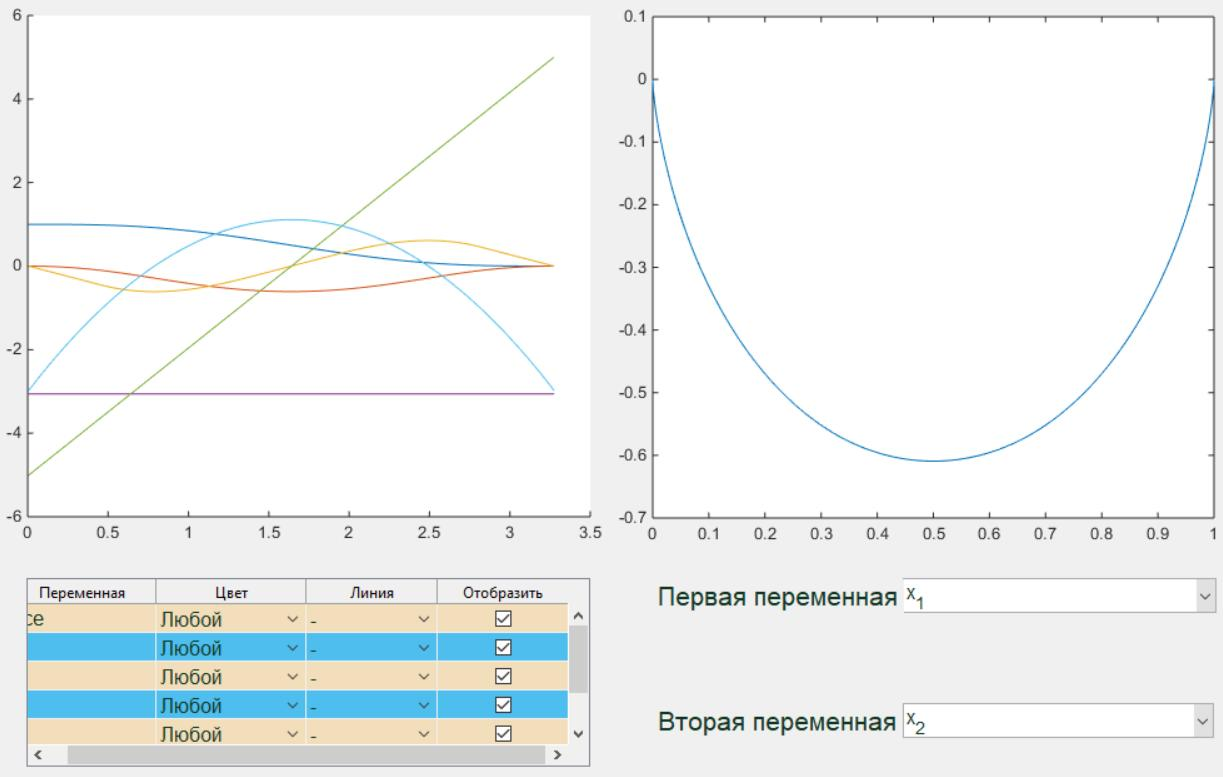
\includegraphics[scale=0.5]{task_3.jpg}}
\caption{Результаты решения задачи <<Функционал типа "энергия" для трёхкратного интегратора>>}\label{ris:task3}
\end{figure}

\newpage

\section{Список литературы}

\begin{enumerate}
    \item Встроенный <<Help>> среды \textit{Matlab 2014b}.
    \item Официальный <<Help>> среды \textit{Matlab}.  \\
    \emph{https://www.mathworks.com/help/matlab/}
    \item Семинары по работе в среде Matlab Дряженкова Андрея Александровича и Аввакумова Сергея Николаевича.
    \item Ю.Н. Киселёв, С.Н. Аввакумов, М.В. Орлов \emph{Оптимальное управление. Линейная теория и приложения} // 2007, Издательский отдел факультета ВМК МГУ имени М.В. Ломоносова, 270.
\end{enumerate}

\end{document}
